\documentclass[twocolumn]{aastex631}

% Packages
\usepackage{microtype}  % ALWAYS!
\usepackage{amsmath}
\usepackage{amsfonts}
\usepackage{amssymb}
\usepackage{multirow}
\usepackage{tikz}
\usepackage{xcolor}
\usepackage{soul}

\definecolor{pink}{RGB}{232,132,161}
\definecolor{yellow}{RGB}{255,213,0}

\newcommand{\kc}[1]{\textcolor{yellow}{\textbf{kc: #1}} }
\newcommand\shadetext[2][]{%
  \setbox0=\hbox{{\special{pdf:literal 7 Tr }#2}}%
  \tikz[baseline=0]\path [#1] \pgfextra{\rlap{\copy0}} (0,-\dp0) rectangle (\wd0,\ht0);% 
  }
\newcommand{\gb}[1]{\shadetext[left color=blue, right color=red, middle color=lime, shading angle=45]{\textbf{g: #1}} }
% \newcommand{\ecite}[1]{\textcolor{pink}{\textbf{: #1}} }
% \newcommand{\e}[1]{\textcolor{yellow}{\textbf{: #1}} }

\newcommand{\remove}[1]{\textcolor{red}{#1}}
\newcommand{\add}[1]{\textcolor{green}{#1}}

\newcommand{\mlg}{\ensuremath{M_{\rm LG}}}
\newcommand{\mmto}{\ensuremath{M_{\rm M31}}}
\newcommand{\mmw}{\ensuremath{M_{\rm MW}}}
\newcommand{\vtan}{\ensuremath{v_\textrm{tan}}}
\newcommand{\vrad}{\ensuremath{v_\textrm{rad}}}
\newcommand{\ms}[1]{\ensuremath{M_{*{#1}}}}
\newcommand{\reflabel}[1]{\ensuremath{^{\mbox{\scriptsize{#1}}}}}
\newcommand{\scsep}{\ensuremath{\rm r_{sep}/r_{vir}}}
\newcommand{\scvel}{\ensuremath{\rm v_{rel}/v_{vir}}}

\newcommand{\paircat}{\textit{Full Pair Catalog}}
\newcommand{\Rvir}{\ensuremath{\rm R_{vir}}}
\newcommand{\Rphys}{\ensuremath{\rm R_{phys}}}
\newcommand{\Rsc}{\ensuremath{\rm R_{sc}}}
\newcommand{\rsep}{\ensuremath{\rm r_{sep}}}

% Style tweaks
% \renewcommand{\twocolumngrid}{\onecolumngrid}
% \setlength{\parindent}{1.1\baselineskip}
% \sloppy\sloppypar\raggedbottom\frenchspacing

%%%%%%%%%%%%%%%%%%%%%%%%%%%%%%%%%%%%%%%%%%%%%%%%%%%%%%%%%%%%%%%%%%%%%%%%%%%%%%%%
\shorttitle{Pair fractions in TNG100}
\shortauthors{Chamberlain et al.}

%%%%%%%%%%%%%%%%%%%%%%%%%%%%%%%%%%%%%%%%%%%%%%%%%%%%%%%%%%%%%%%%%%%%%%%%%%%%%%%%
\graphicspath{{./}{../plots/}}
% Missions
\newcommand{\project}[1]{\textsl{#1}}

% Packages / projects / programming
\newcommand{\package}[1]{\textsl{#1}}
\newcommand{\acronym}[1]{{\small{#1}}}
\newcommand{\github}{\package{GitHub}}
\newcommand{\python}{\package{Python}}
\newcommand{\astropy}{\package{Astropy}}

% Stats / probability
\newcommand{\given}{\,|\,}
\newcommand{\norm}{\mathcal{N}}
\newcommand{\pdf}{\textsl{pdf}}

% Maths
\newcommand{\dd}{\mathrm{d}}
\newcommand{\transpose}[1]{{#1}^{\mathsf{T}}}
\newcommand{\inverse}[1]{{#1}^{-1}}
\newcommand{\argmin}{\operatornamewithlimits{argmin}}
\newcommand{\mean}[1]{\left< #1 \right>}

% Non-scalar variables
\renewcommand{\vec}[1]{\ensuremath{\bs{#1}}}
\newcommand{\mat}[1]{\ensuremath{\mathbf{#1}}}

% Unit shortcuts
\newcommand{\Msun}{\ensuremath{\mathrm{M}_\odot}}
\newcommand{\Mjup}{\ensuremath{\mathrm{M}_{\mathrm{J}}}}
\newcommand{\kms}{\ensuremath{\mathrm{km}~\mathrm{s}^{-1}}}
\newcommand{\pc}{\ensuremath{\mathrm{pc}}}
\newcommand{\kpc}{\ensuremath{\mathrm{\,kpc}}}
\newcommand{\Mpc}{\ensuremath{\mathrm{Mpc}}}
\newcommand{\kmskpc}{\ensuremath{\mathrm{km}~\mathrm{s}^{-1}~\mathrm{kpc}^{-1}}}
\newcommand{\dayd}{\ensuremath{\mathrm{d}}}
\newcommand{\yr}{\ensuremath{\mathrm{yr}}}
\newcommand{\Myr}{\ensuremath{\mathrm{Myr}}}
\newcommand{\Gyr}{\ensuremath{\mathrm{\,Gyr}}}
\newcommand{\Kel}{\ensuremath{\mathrm{K}}}
\newcommand{\masyr}{\ensuremath{\mathrm{mas}~\mathrm{yr}^{-1}}}
\newcommand{\muasyr}{\ensuremath{\mu\mathrm{as}~\mathrm{yr}^{-1}}}

% Misc.
\newcommand{\bs}[1]{\boldsymbol{#1}}

% Astronomy
\newcommand{\DM}{{\rm DM}}
\newcommand{\feh}{\ensuremath{{[{\rm Fe}/{\rm H}]}}}
\newcommand{\df}{\acronym{DF}}

% TO DO
\newcommand{\todo}[1]{{\color{red} TODO: #1}}
\newcommand{\apw}[1]{{\color{blue} APW says: #1}}

% Projects
\newcommand{\gaia}{\textsl{Gaia}}
\newcommand{\gaiadr}{\textsl{Gaia}~\acronym{EDR3}}
\newcommand{\hst}{\textsl{HST}}

% Paper specific
\newcommand{\paircat}{\textit{Full Pair Catalog}}

\newcommand{\lcdm}{\ensuremath{\Lambda \rm CDM}} 
\newcommand{\sublink}{\textsc{sublink}} 
\newcommand{\subfind}{\textsc{subfind}} 

% masses - halo
\newcommand{\Mpeak}{\ensuremath{M_{\mathrm{peak}}}}
\newcommand{\Mhalo}{\ensuremath{M_{\mathrm{h}}}}
\newcommand{\MG}{\ensuremath{\rm M_{\mathrm{G}}}}
\newcommand{\mlg}{\ensuremath{M_{\rm LG}}}

% masses - stellar
\newcommand{\Ms}{\ensuremath{\rm M_{{*}}}}
\newcommand{\msam}{\ensuremath{M_{*,\mathrm{am}}}}
\newcommand{\mssim}{\ensuremath{M_{*,\mathrm{sim}}}}
\newcommand{\ms}[1]{\ensuremath{M_{*{#1}}}}

\newcommand{\vtan}{\ensuremath{v_\textrm{tan}}}
\newcommand{\vrad}{\ensuremath{v_\textrm{rad}}}
\newcommand{\reflabel}[1]{\ensuremath{^{\mbox{\scriptsize{#1}}}}}

\newcommand{\Rvir}{\ensuremath{\rm R_{vir}}}
\newcommand{\Rphys}{\ensuremath{\rm R_{phys}}}
\newcommand{\Rsc}{\ensuremath{\rm R_{sc}}}
\newcommand{\rsep}{\ensuremath{\rm r_{sep}}}

% Affiliations
\newcommand{\affuofa}{University of Arizona, 933 N. Cherry Ave,
    Tucson, AZ 85721, USA}

\newcommand{\affuofu}{Department of Astronomy, University of Utah, Salt Lake City, UT 84112, USA}

\begin{document}

\title{Orbits
}

\author[0000-0001-8765-8670]{Katie~Chamberlain}
\affiliation{\affuofa}

\author[0000-0002-9820-1219]{Ekta~Patel}
\thanks{Hubble Fellow}\affiliation{\affuofu}


\author[0000-0003-0715-2173]{Gurtina Besla}
\affiliation{\affuofa}




\author{others}

\begin{abstract}

\end{abstract}

%%%%%%%%%%%%%%%%%%%%%%%%%%%%%%%%%%%
\section{Introduction} \label{sec:intro}

$z=1.5$ corresponds to snapshot \#40 in the TNG sim
% Introduce RG15, Lotz, etc.


%%% OUTLINE
\section{Sample Data}
%recap last paper and mention which data sample we narrow down to (low mass major pairs only) -- give examples of orbits

\subsection{Isolated Pairs}
We utilize the \paircat{} of isolated low and high mass pairs described in ~\citet{Chamberlain2024}. 
In summary, the \paircat{} is a collection of isolated subhalo pairs at each snapshot of the highest resolution run of the $(110.7\,\Mpc)^3$ volume IllustrisTNG simulation, TNG100-1 (hereafter TNG100). 

Stellar masses were assigned to Abundance matching 
For the purposes of our study, we will only be using the 


\subsubsection{brief recap of last paper}
\texttt{SUBLINK} algorithm~\citep{RG2015}

\subsubsection{Assumption of Isolation}
% justify stuff from last paper

\subsection{Mergers and Orbits}
\subsubsection{Calculation of merger fraction of total sample}
Plot \#1: Merger fraction either before or after orbits
Note that it is very interesting that dwarf pairs in the field have high merger fractions, while the likelihood of merger is very low in more dense environments (add citation).



\subsubsection{Pulling Orbits}
Orbital data for each pair from the \paircat{} was collected by following each subhalo of the pair both forwards and backwards in time via the \texttt{SUBLINK} algorithm~\citep{RG2015} merger trees.


The infall snapshot is defined as ZZZ. 
We will define the "First Infall" as the first snapshot where the primary and secondary have the same parent FoF halo. 

Mergers are XXX 
Non-mergers are YYY. 
The merger snapshot is defined ALALAL.

The orbit collection includes mergers and non-mergers, which 

Plot \#2: Orbits plot
Figure~\ref{fig:example-orbits} shows a collection of example orbits pulled from the merger trees of low-mass major pairs initially selected at $z=2$. 

 Non-mergers: These orbits can have a variety of orbital periods and thus, a number of different pericentric passages. The two lighter blue orbits are very long period orbits with 1-2 pericenter passages in the past 10Gyr, while the darker blue orbits has a much shorter period with many close encounters throughout, and 3 close passages in just the past 2 Gyr.

Mergers:  Pairs chosen at $z=2$ on average merge at $z=XX$/within XX Gyrs, though the spread of merger timescales is large, leading to a single redshift-selected sample having merger timescales between 0.5-8Gyr.

Flybys:

\subsubsection{Interpolation}
\begin{figure}[htb]
    \centering
    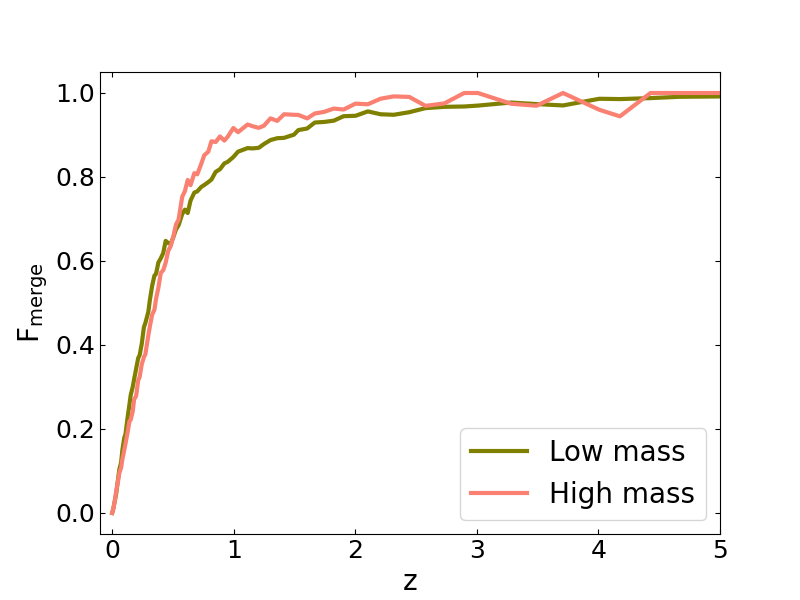
\includegraphics[width=\columnwidth]{plots/bet-on-it/1_fmerge_comp.png}
    \caption{The fraction of pairs that merge before z=0 as a function of the redshift where they were selected via the selection criteria for the \paircat{} from \citet{Chamberlain2024}. At $z>1$, the fraction of selected pairs that merge before $z=0$ is upwards of 80\% for both low mass and high mass isolated pairs. The sharp decline to $F_{\rm merge}$ at $z=0$ is a non-physical feature of the simulation ending at $z=0$, thus unable to follow the pairs after the simulation ends to see what fraction of pairs may have merged.}
    \label{fig:fmerge}
\end{figure}

\begin{figure}[htb]
    \centering
    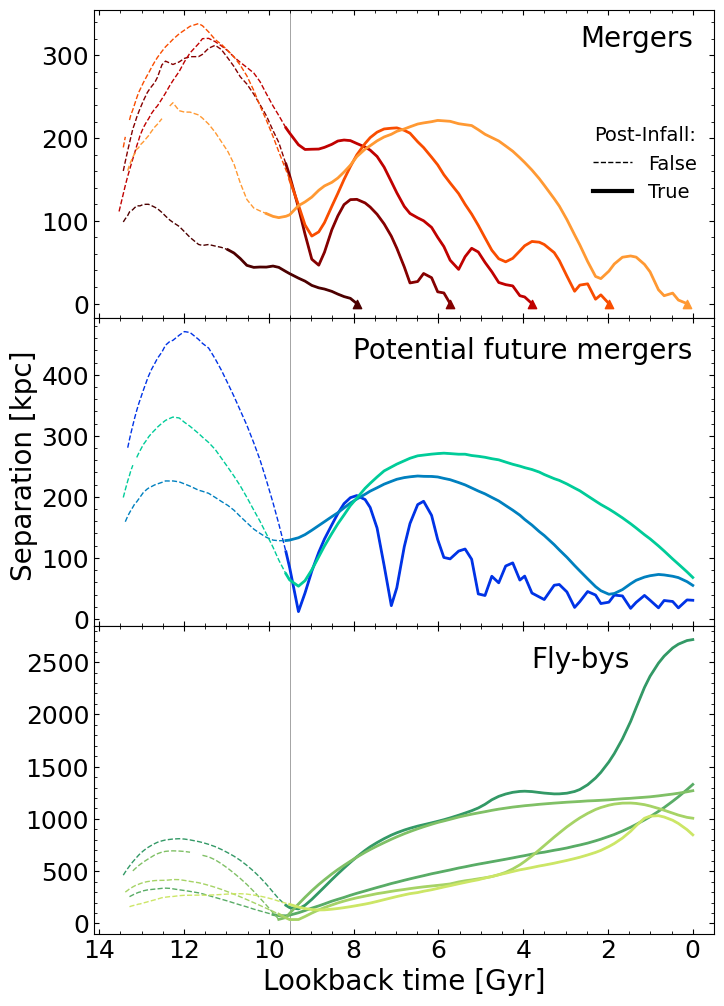
\includegraphics[width=\columnwidth, trim={0.4cm 1.75cm 1cm 3.5cm}, clip]{plots/bet-on-it/5_exampleorbits.png}
    \caption{Selection of example orbits of low-mass major pairs selected at $z=1.5$, showing the separation between the primary and secondary halo of the pair as a function of Lookback Time. The vertical grey line marks $z=1.5$ at a Lookback Time of $9.5\,\Gyr$.
    Solid lines represent the parts of the orbit where the primary and secondary halo have the same FoF group, while the dashed lines show where they are not within the same FoF group. 
    (Top) Orbits of pairs that merge before $z=0$. Pairs chosen at $z=1.5$ on average merge at \kc{$z=XX$/within XX Gyrs}.
    (Middle) Orbits of pairs that did not merge before $z=0$ (non-mergers), but are likely to merge if the simulation continued. 
    (Bottom) Orbits of pairs that did not merge before $z=0$ (non-mergers) and are unlikely to do so in the future $\sim2\Gyr$ (past the end of the simulation). 
    }
    \label{fig:example-orbits}
\end{figure}

\begin{figure*}[htb]
    \centering
    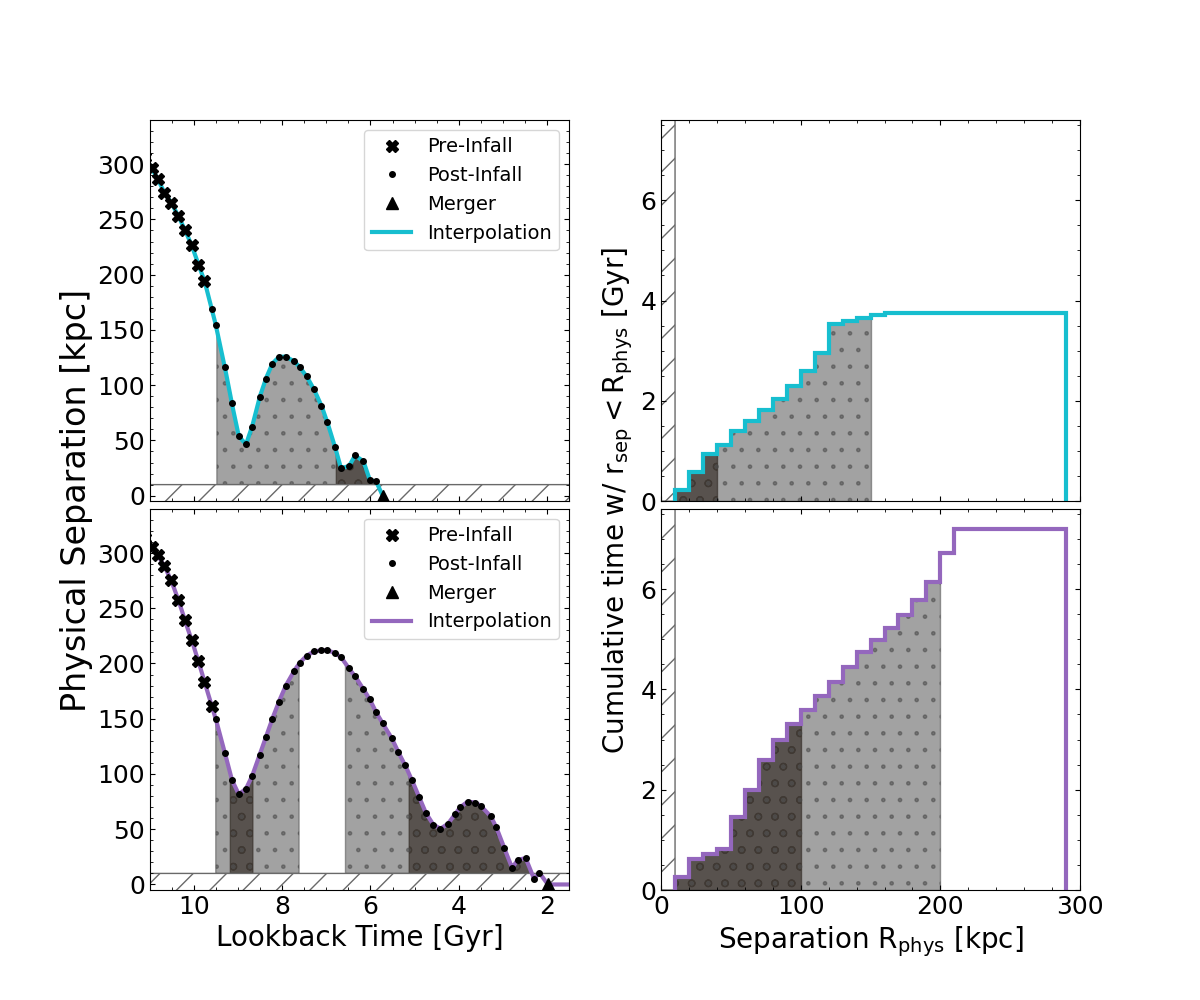
\includegraphics[width=0.8\textwidth]{plots/bet-on-it/4_examplecombo_unlabeled.png}
    \caption{ Caption    }
    \label{fig:interpolation}
\end{figure*}



% ###########################################################################################
% Results II 
% ###########################################################################################

\section{Results - The Mass Dependence of Merger Timescales}
% The point of this subsection: to show that using the same "observability times" for pairs selected in the same physical separation bins wouldn't work, and that the selection criteria for close pairs should either be scaled by size of halo, OR that timescales for ow mass and high mass would be different by a lot for the same physical separation choices. (Maybe come up with a functional form to relate the two? )
\subsection{explain subset of data used for this section}
\subsection{Cumulative time}
Plot \#3: Cumulative time example calculation plot
\subsection{"time til merger" for selected snapshots for LvH. }
Maybe also (distribution plot 2D hist? as function of selected separation)
\subsection{Cumulative distributions}
\subsubsection{Physical}
Plot \#4: Cumulative distribution, low mass vs. high mass
\subsubsection{Scaled}
Plot \#5: Cumulative distribution in scaled units, low mass vs. high mass
Plot \#3-5?: the cumulative with spread for low vs. high mass

\begin{figure*}[htb]
    \centering
    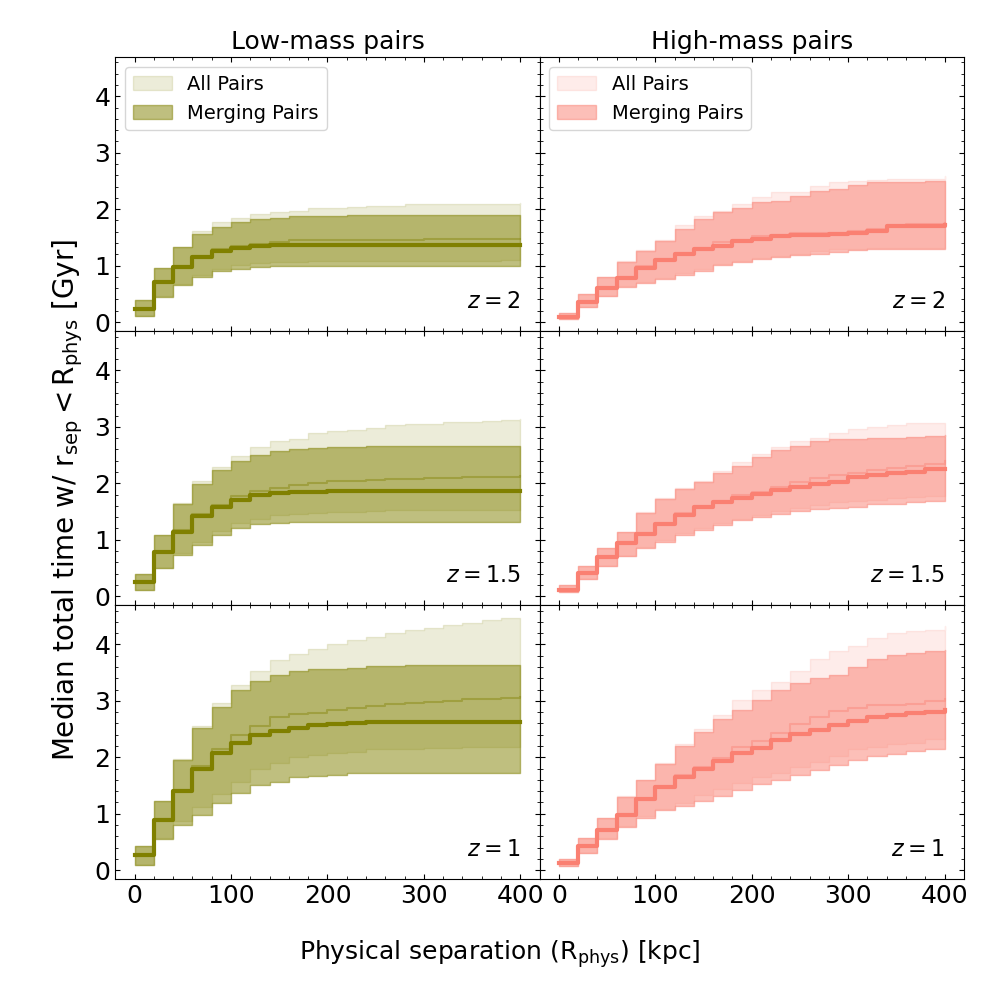
\includegraphics[width=\textwidth]{plots/bet-on-it/2_medtotal_LoHi.png}
    \caption{\kc{reverse the direction of z} 
    The median (solid) and 1st-3rd quartile spread (shaded regions) of the cumulative time that isolated low-mass pairs (left) and high-mass pairs (right) spend with separations \rsep{} between $10\kpc$ and \Rphys{}. 
    The Merging Pairs sample (dark green and dark pink) selected at $z=(1,1.5,2)$ merge before $z=0$, while the All Pairs sample (light green and light pink) include all the pairs from the \paircat{} (mergers and non-mergers).  
    The low-mass (high-mass) merging pairs represent XX\%(XX\%) of the low-mass (high-mass) pair sample at $z=1,1.5, \mbox{and } 2$ respectively. 
    The sample of All Pairs spend more time at higher separations than the merging pairs, as expected since the non-merging pairs are not likely to have very low separations that would result in mergers prior to $z=0$. 
    For a more direct comparison between the low-mass and high-mass pairs, see Fig.~\ref{fig:phys-vs-scaled}. 
    }
    \label{fig:low-vs-high}
\end{figure*}

\begin{figure*}[htb]
    \centering
    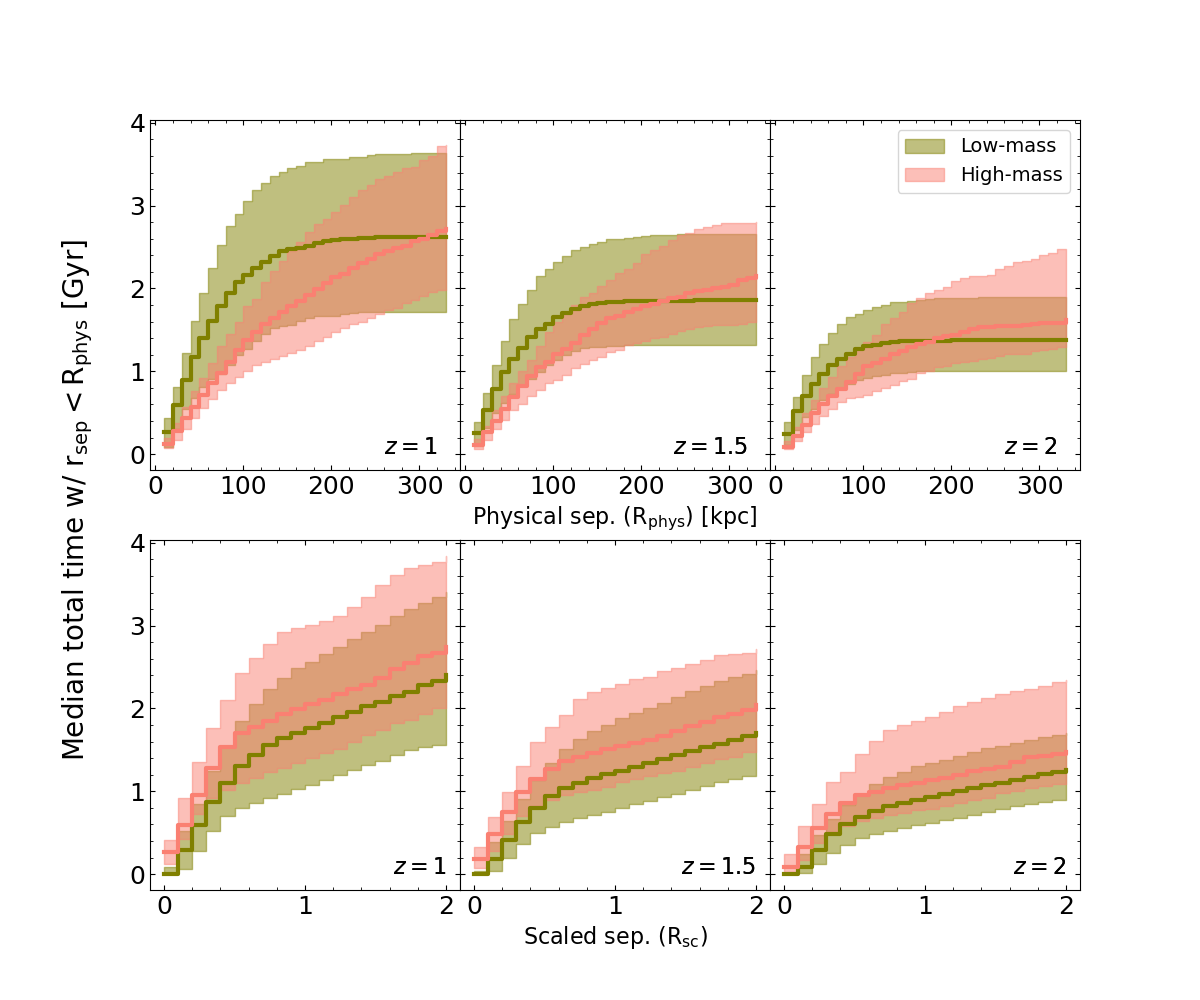
\includegraphics[width=\textwidth]{plots/bet-on-it/2_medtotal_PhScT.png}
    \caption{\kc{Add legend to plot, and I think reverse the direction of z} 
    The median and 1st-3rd quartile spread of the cumulative time that isolated merging pairs, selected at $z=(1,1.5,2)$, spend with separations \rsep{} greater than $10\kpc$ and less than either \Rphys{} or \Rsc{}.
    %
    (Top) The median total time spent by isolated merging pairs with separations between $10\kpc$ and \Rphys{}.
    Low-mass pairs spend a longer amount of time within $\sim200\kpc$ than high-mass pairs at each of these redshifts. 
    However, high-mass galaxies spend more time at higher separations of $\rsep>200-300\kpc$. This is because the elapsed time is measured starting at the infall snapshot of the pair, and high-mass halos have larger radii, the high-mass halo orbits have a broader distribution of separations that extend to larger separations than those of the low-mass pairs.
    (Bottom) The median total time spent by pairs with separations greater than $\rsep>10\kpc$ and less than a given fraction of the virial radius ($\rsep/\Rvir<\Rsc$) of the pair, which scales with mass and redshift.  
    High-mass pairs spend more time within the same scaled separation than low-mass pairs. For example, a high-mass pair selected from the $z=1.5$ sample will spend \kc{XXGyr} within \kc{$1\Rsc\sim XX\kpc$}, while a low-mass pair from the same sample will spend \kc{XXGyr} within \kc{$1\Rsc\sim XX\kpc$}. 
    Low-mass and high-mass pairs have similar cumulative time profiles as a function of scaled separation, with a roughly constant offset for all scaled separations. 
    The high-mass pairs spend a median of \kc{$XX\Gyr$} more than low-mass pairs at every scaled separation at $z=1$ and $z=1.5$, and a median of \kc{$XX\Gyr$} more $z=2$.
    }
    \label{fig:phys-vs-scaled}
\end{figure*}



% ###########################################################################################
% Results II 
% ###########################################################################################
\section{Results - The Redshift Dependence of Merger Timescales}
% point: to show that the amount of time that pairs spend in the same physical separation bins changes by a significant amount between high and low redshift. In order to do pair fraction-merger rate studies appropriately, use Tobs(z), as suggested in Snyder 2017.  
\subsection{explain subset of data used for this section}
\subsection{explain how data in the plot was calculated}
\subsection{Redshift dependence}
Plot \#6: Redshift dependence for low and high mass pairs
\subsection{Best fit redshift dependence?/scaling?}
Is $(1+z)^-2$ the best fit? 


\begin{figure*}[htb]
    \centering
    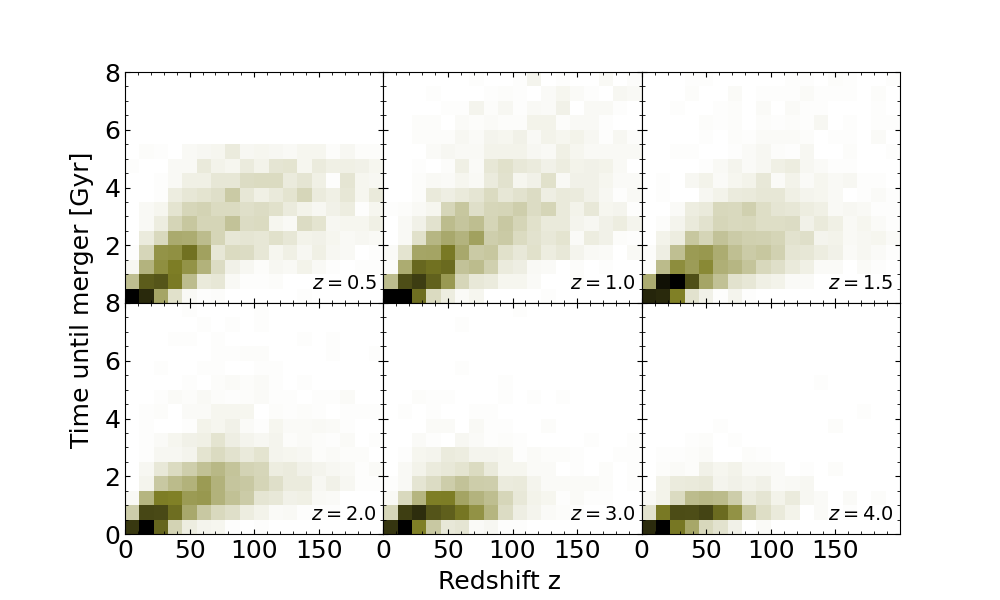
\includegraphics[width=\textwidth]{plots/bet-on-it/3_Timevsseplow-2d.png}
    \caption{}
    \label{fig:low-vs-high}
\end{figure*}

\begin{figure*}[htb]
    \centering
    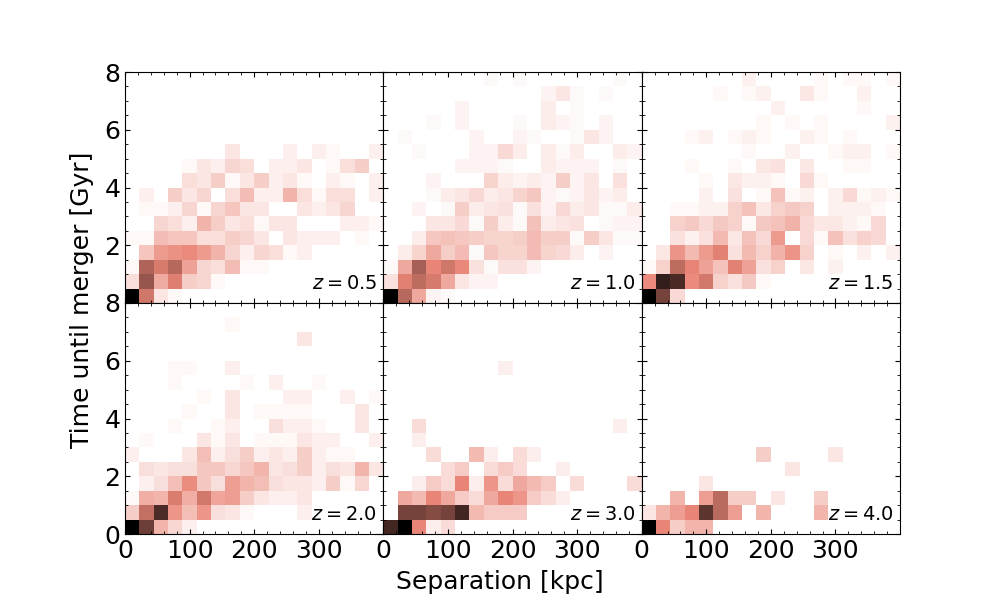
\includegraphics[width=\textwidth]{plots/bet-on-it/3_Timevssephigh-2d.png}
    \caption{}
    \label{fig:low-vs-high}
\end{figure*}
\begin{figure*}[htb]
    \centering
    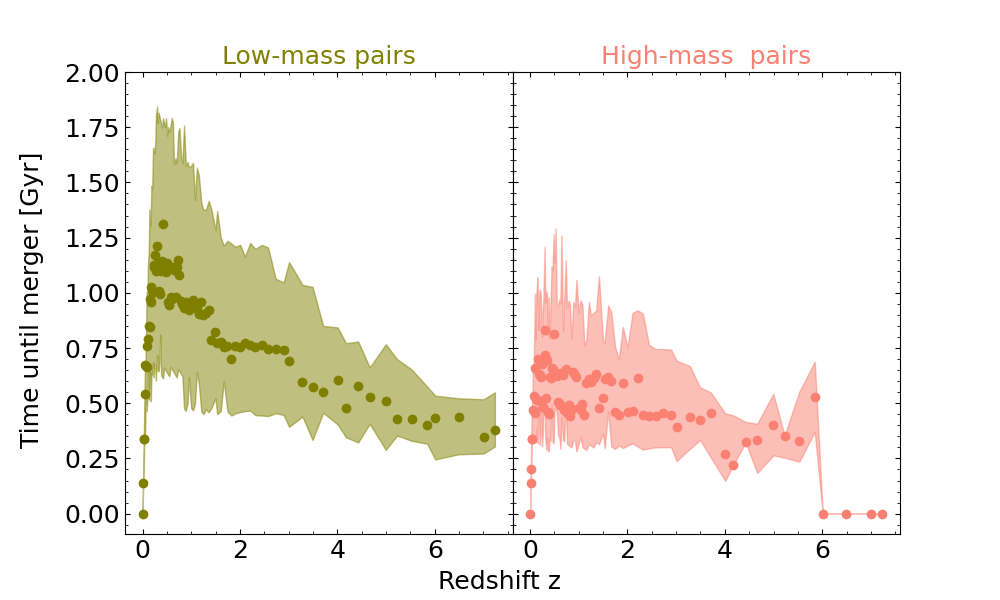
\includegraphics[width=\textwidth]{plots/bet-on-it/3_Timevsz.png}
    \caption{}
    \label{fig:low-vs-high}
\end{figure*}
\begin{figure*}[htb]
    \centering
    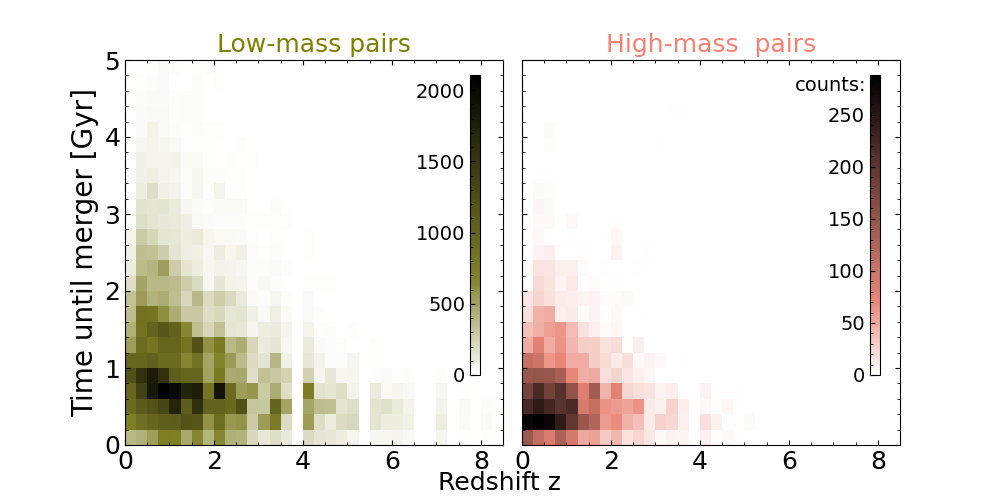
\includegraphics[width=\textwidth]{plots/bet-on-it/3_Timevsz-2d.png}
    \caption{}
    \label{fig:low-vs-high}
\end{figure*}



% \section{Discussion}
% \subsection{Merger Rates for Dwarf Pairs}
% % - What combination of values best reproduces the merger fraction acquired from the sims?
% % Do you need the scale of merger probability as in Ventou to get the match?
% % Vicente & Casteels 2014 comparison (pair fractions plot)
% \subsection{Pairs of Dwarfs That Do Not Merge}
% % can talk about the unmerged fraction merger rates here
% \subsection{Choosing Samples at Lower and Higher Redshift}
% % can also compare to samples to merger fractions and merger rates chosen at z=1 and z=2 (plots you have already)
% \subsection{Comparing with Merger Rates for Massive Galaxy Pairs}
% % compare to massive pairs in both obs window and merger rate
% % compare back to the assumption of isolation
\section{Summary and Conclusions}

% To do:
% -Sample: starting with FoF group cut and always show the total sample (merged and unmerged) since the unmerged sample is so small
% -Keep Fig 1: (two panels) add in a few more orbits to show the diversity and then have a panel to show one example where you shade everything below 100 kpc to show how the total time at S is computed
% -Keep Figure 2 as is 
% -Remove Figure 3
% -Figure 4: remove normalization of both samples so it's clear that the unmerged ones spend a lot of time at high separation and that they are a small percent of the fraction (put this in discussion or an appendix)
% -Remove Fig 5 and state conclusions in words along with the FoF group selection (most pairs have been in the same group for 1.5 Gyr) (can quote percentages from a cumulative version of the plot, or sum)
% -Figure 6: only show the *full* sample with the FoF group cut 
% check the half mass radius of the most massive dwarfs in your sample and justify 10 kpc by saying you want to be able to resolve twice that 









% \section{Discussion}

** 
\appendix
\begin{figure}[htb]
    \centering
    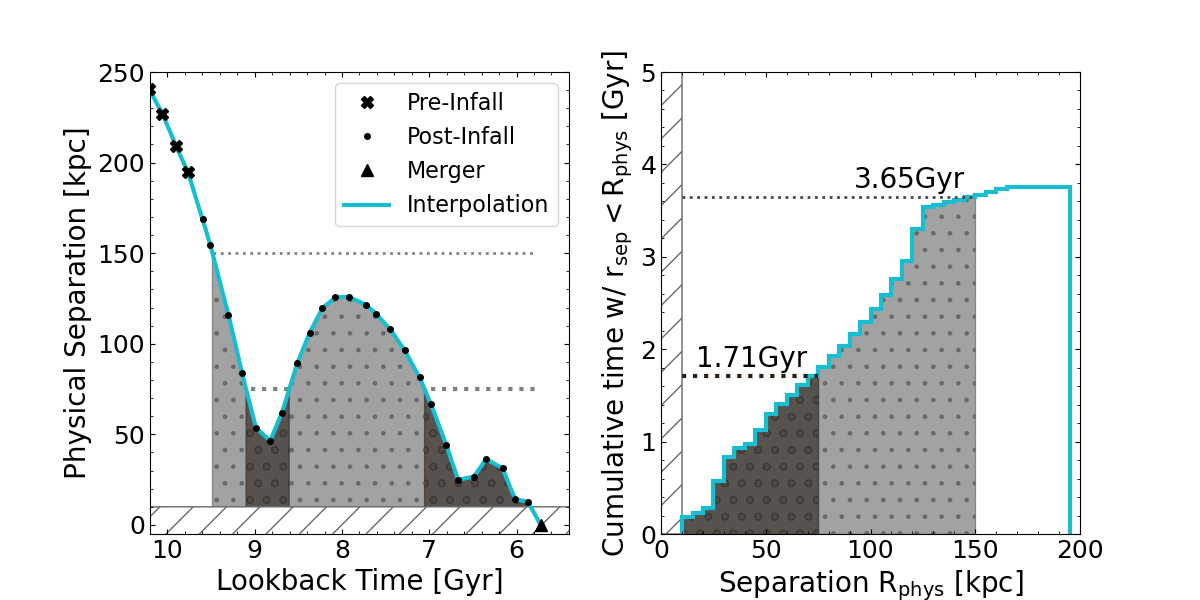
\includegraphics[width=0.5\columnwidth]{plots/bet-on-it/4_example1.png}
\end{figure}
\begin{figure}[htb]
    \centering
    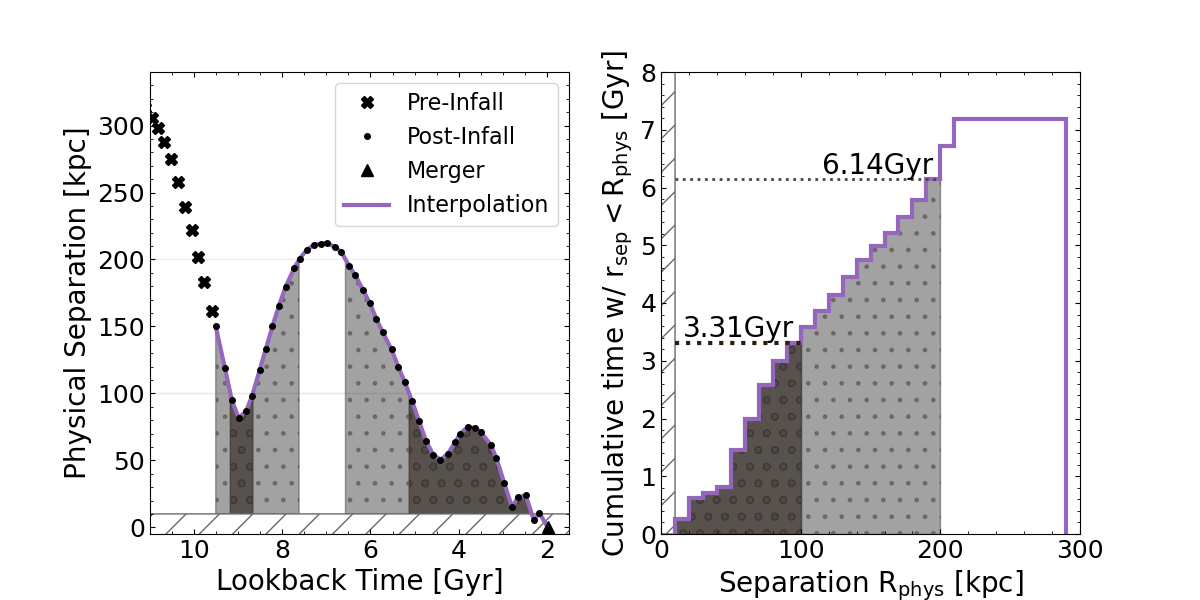
\includegraphics[width=0.5\columnwidth]{plots/bet-on-it/4_example2.png}
    \caption{}
\end{figure}
\begin{figure}[htb]
    \centering
    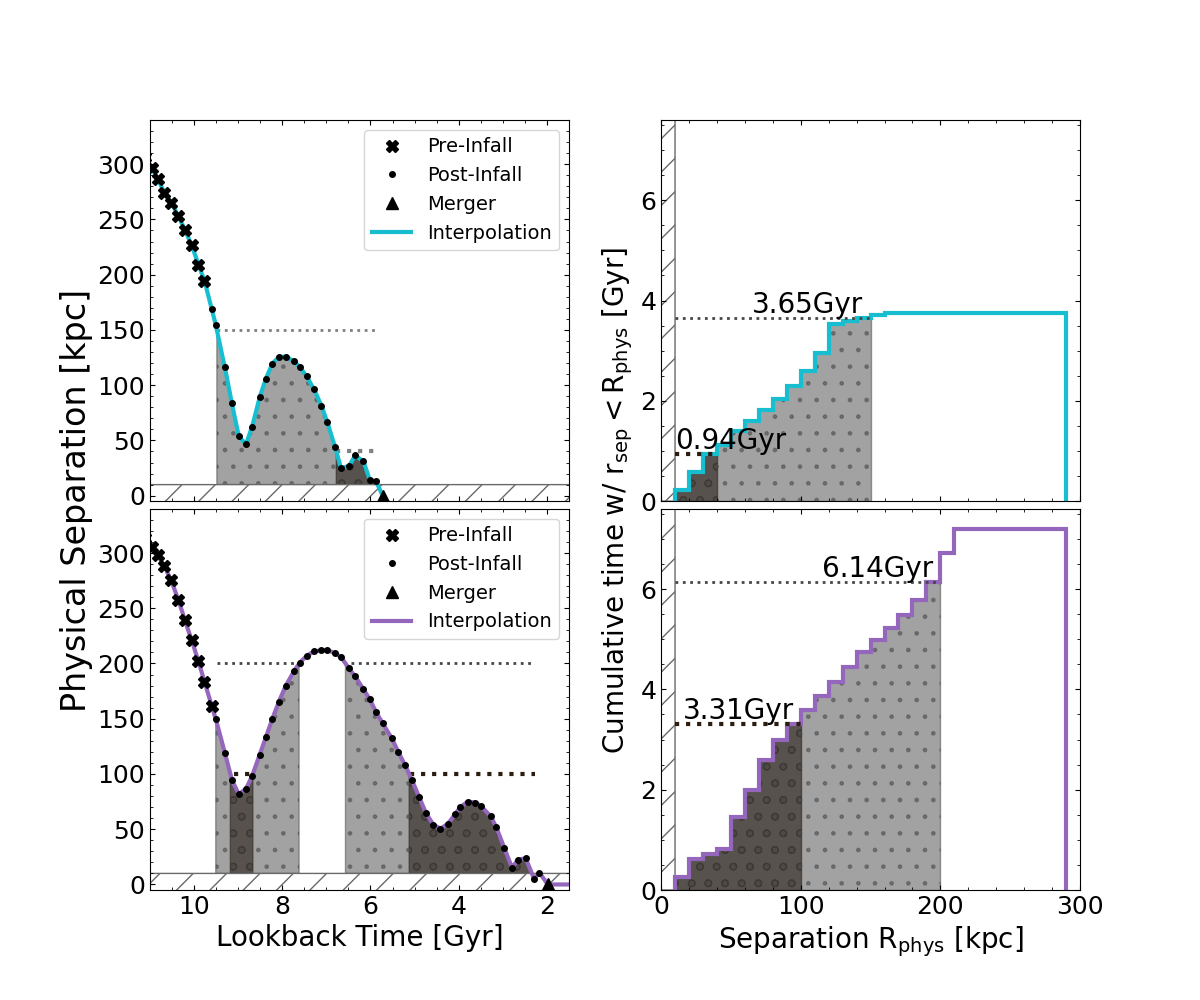
\includegraphics[width=0.5\columnwidth]{plots/bet-on-it/4_examplecombo.png}
\end{figure}
\begin{figure}[htb]
    \centering
    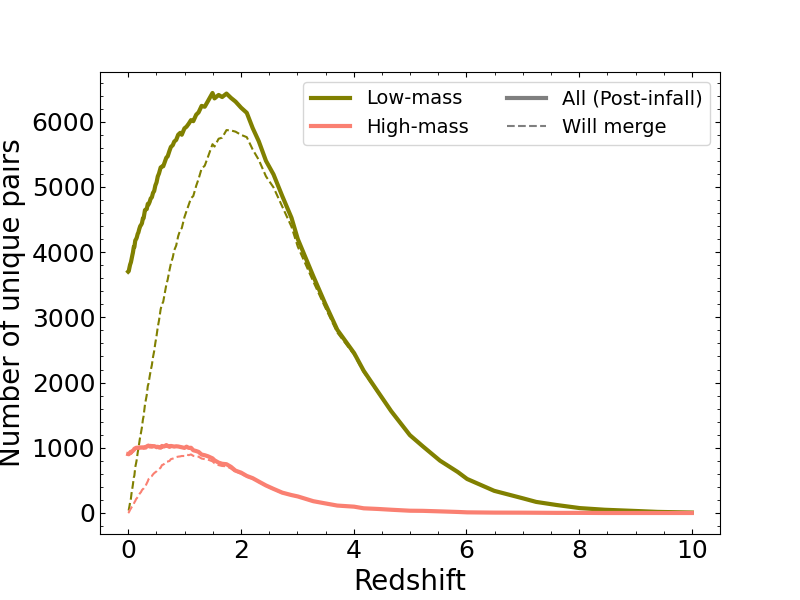
\includegraphics[width=0.5\columnwidth]{plots/bet-on-it/3_number_pairs.png}
\end{figure}
\begin{figure}[htb]
    \centering
    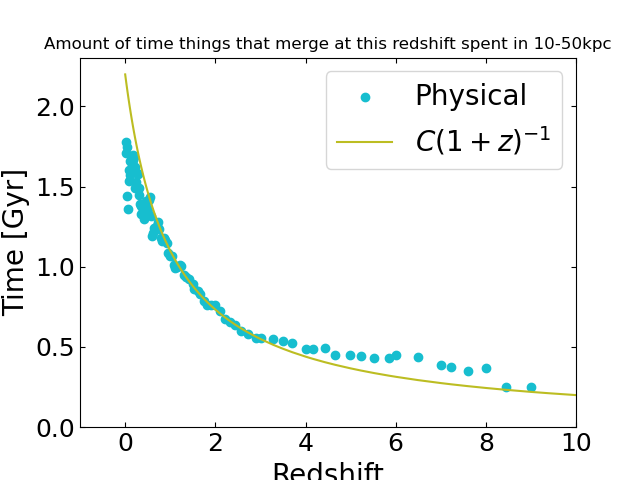
\includegraphics[width=0.5\columnwidth]{plots/bet-on-it/3_timeinbin_beforemerger.png}
\end{figure}
\begin{figure}[htb]
    \centering
    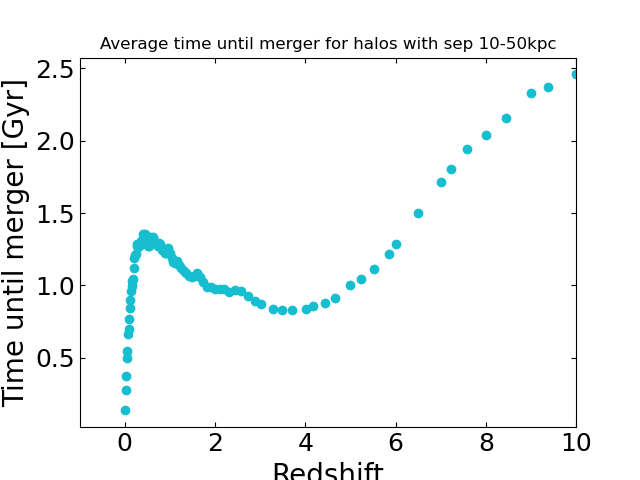
\includegraphics[width=0.5\columnwidth]{plots/bet-on-it/3_timeinbin_untilmerger_phys.png}
\end{figure}

% \begin{figure*}[htb]
%     \centering
%     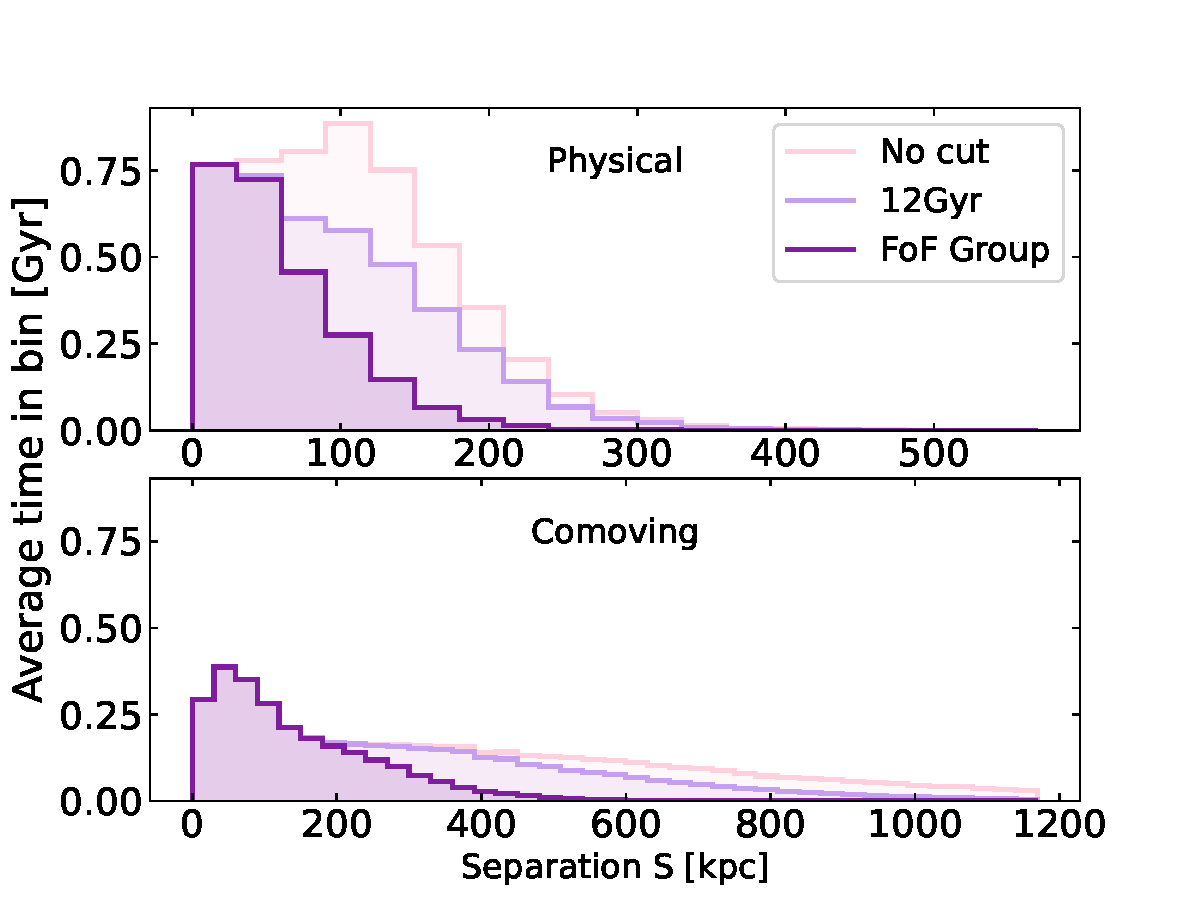
\includegraphics[width=\columnwidth]{plots/4_timescales/timevssep_phys+co.pdf}
%     \caption{}
%     % \label{fig:phys-comoving}
% \end{figure*}

% \begin{figure*}[htb]
%     \centering
%     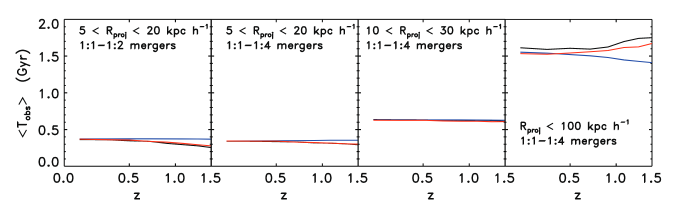
\includegraphics[width=\columnwidth]{lotz.png}
%     \caption{}
%     % \label{fig:phys-comoving}
% \end{figure*}







\bibliography{refs}{}
\bibliographystyle{aasjournal}

\end{document}

